% *********************************************************************
% © 2021–2026 Jeremy Sylvestre
%
% Permission is granted to copy, distribute and/or modify this document
% under the terms of the GNU Free Documentation License, Version 1.3 or
% any later version published by the Free Software Foundation; with no
% Invariant Sections, no Front-Cover Texts, and no Back-Cover Texts. A
% copy of the license is included in the appendix entitled “GNU Free
% Documentation License” that appears in the output document of this
% PreTeXt source code. All trademarks™ are the registered® marks of
% their respective owners.
%
% *********************************************************************

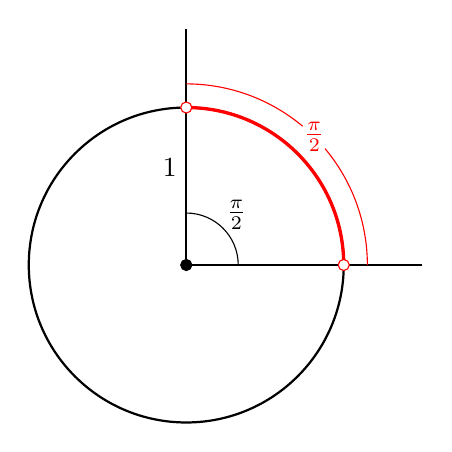
\begin{tikzpicture}
[
	closedpt/.style={circle,draw,fill,inner sep=0pt,minimum size=4pt},
	openpt/.style={circle,draw,inner sep=0pt,minimum size=4pt},
	scale=2
]

	\node[closedpt] at (0,0) (o) {};

	\draw[thick] (o) -- (1.5,0);
	\draw[thick] (o) -- (0,1.5);

	\draw[thick] (1,0) arc (0:360:1cm);
	\draw[red,very thick] (1,0) arc (0:90:1cm);
	\draw[white,fill=white] (1,0) circle (0.03cm);
	\node[openpt,red] at (1,0) (r) {};
	\draw[white,fill=white] (0,1) circle (0.03cm);
	\node[openpt,red] at (0,1) (r2) {};

	\draw[dashed,very thin] (o) to node[above left] {$1$} (r2);

	\node[red] at (0.813,0.813) {$\frac{\pi}{2}$};
	\draw[red] (1.15,0) arc (0:40:1.15cm);
	\draw[red] (0,1.15) arc (90:50:1.15cm);

	\draw (0.33,0) arc (0:90:0.33);
	\node at (0.318,0.318) {$\frac{\pi}{2}$};

\end{tikzpicture}
